\documentclass[a4paper,12pt]{article}
\usepackage[utf8]{inputenc}
\usepackage[T2A]{fontenc}
\usepackage[russian,english]{babel}
\usepackage[pdftex]{graphics}
\DeclareGraphicsExtensions{.pdf,.png,.jpg}
\graphicspath{{pictures/}}
\begin{document}
\begin{center}
Санкт-Петербургский государственный политехнический университет
\\Кафедра компьютерных систем и программных технологий
\end{center}
\vspace*{10em plus .6em minus .5em}

\begin{center}
{\LARGEТелекоммуникационные технологии
\\Лабораторная работа №7
\\Помехоустойчивое кодирование}
\end{center}

\vspace*{5em plus .6em minus .5em}
\begin{flushright}
Выполнил:\\студент гр.33501/4\\Курякин Д. А.\\Проверила:\\Богач Н.В.
\end{flushright}

\vspace*{15em plus .6em minus .5em}
\begin{center}
{\smallСанкт-Петербург
\\2018}
\end{center}
\pagestyle{empty}
\newpage
\pagestyle{plain}


\section{Цель}

Изучение методов помехоустойчивого кодирования и сравнение их свойств

\section{Постановка задачи}

\begin{itemize}
\item Провести кодирование/декодирование сигнала, полученного с помощью функции randerr кодом Хэмминга 2-мя способами: с помощью встроенных функций encode/decode, а также через создание проверочной и генераторной матриц и вычисление синдрома. Оценить корректирующую способность кода.
\item Выполнить кодирование/декодирование циклическим кодом, кодом БЧХ, кодом Рида-Соломона. Оценить корректирующую способность кода.
\end{itemize}

\section{Теоретическое обоснование}

Обычно в процессе кодирования информация преобразуется из формы, удобной для непосредственного использования, в форму, удобную для передачи, хранения или автоматической обработки. В более узком смысле кодированием информации называют представление информации в виде кода. Средством кодирования служит таблица соответствия знаковых систем, которая устанавливает взаимно однозначное соответствие между знаками или группами знаков двух различных знаковых систем.
Декодирование — это процесс, обратный процессу кодирования, процесс выявления первоначального смысла, исходной идеи отправителя, понимания смысла его сообщения.

Циклический код — подкласс линейных кодов, обладающие следующим свойством: циклическая подстановка символов в кодированном блоке дает другое возможное кодовое слово того же кода.

К циклическим кодам относятся коды Хэмминга, которые являются одним из немногочисленных примеров совершенных кодов. Длина кодированного блока равна 2m-1. Порождающая и проверочная матрицы для кодов Хэмминга генерируются функцией hammgen. 

Среди циклических кодов широкое применение нашли коды Боуза-Чоудхури-Хоквингема (БЧХ). Для работы с ними есть функции bchenco (кодирование) и bcddeco (декодирование). Функция bchpoly позволяет расчитывать и считывать параметры или порождающий полином для двоичных кодов БЧХ.

Частным случаем БЧХ кодов являются коды Рида-Соломона - подкласс циклических блочных кодов. Это единственные поддерживаемые пакетом Communications недвоичные коды. Для работы с этим кодом есть функции rsenco (кодирование) и rsdeco (декодирование). Функции rsencof и rsdencof осуществляют кодирование и декодирование текстового файла. Функция rspoly генерирует порождающие полиномы для кодов Рида-Соломона.
\newpage

\section{Ход работы}
\begin{enumerate}
	{\itemРезультат кодирования/декодирования кодом Хэмминга с использованием стандартных функций:
		{\center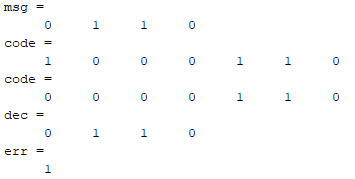
\includegraphics{./pictures/1.png} \\ Рис.1 Результат работы программы}
		\\}
	
	{\itemРезультат кодирования/декодирования кодом Хэмминга с использованием проверочной и генераторной матриц и вычисление синдрома:
		\center{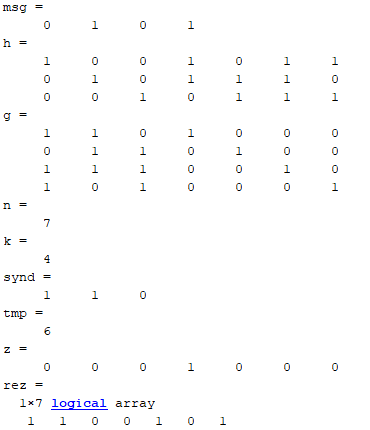
\includegraphics{./pictures/2.png} \\ Рис.2 Результат работы программы}
		\\}
	
	{\itemРезультат кодирования/декодирования циклическим кодом:
		\center{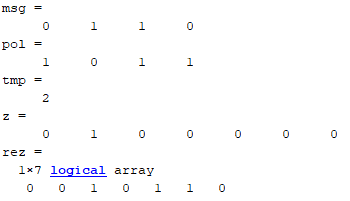
\includegraphics{./pictures/3.png} \\ Рис.3  Результат работы программы}
		\\}
	
	{\itemРезультат кодирования/декодирования кодом БЧХ:
		\center{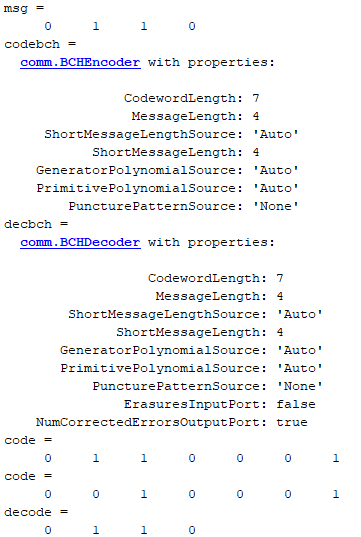
\includegraphics{./pictures/4.png} \\ Рис.4 Результат работы программы}
		\\}
	
	{\itemРезультат кодирования/декодирования кодом Рида-Соломона:
		\center{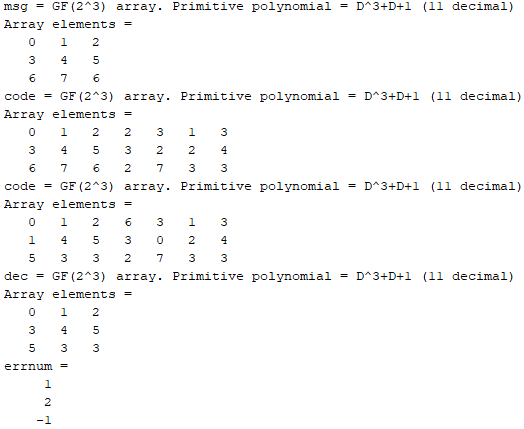
\includegraphics{./pictures/5.png} \\ Рис.5 Результат работы программы}
		\\}
	
\end{enumerate}

\section{Вывод}

В ходе данной работы были получены навыки кодирования цифровых сигналов. Кодирование таких сигналов происходит по принципу избыточности. Каждый из исследованных кодов имеет свои преимущества и недостатки, поэтому использование конкретного из них должно быть обусловлено постановкой определенной задачи. Код Хэмминга достаточно простой в использовании, не требует больших мощностей. Однако он может исправить только одну допущенную ошибку в переданном сообщении. Код Рида-Соломона способен исправлять несколько ошибок, так же он может оперировать десятичными числами, а не только двоичными.

\end{document}
